\documentclass[10pt,a4paper]{article}
\usepackage[margin=18mm,top=16mm,bottom=17mm]{geometry}
\usepackage[T1]{fontenc}
\usepackage{lmodern}
\usepackage{amsmath,amssymb,booktabs,graphicx,xcolor,caption,microtype,array,enumitem,tikz,float}
\usepackage[colorlinks=true,linkcolor=black,citecolor=black,urlcolor=black]{hyperref}
\usetikzlibrary{arrows.meta,positioning,calc}

\definecolor{paperc}{RGB}{213,94,0}   % Paper network (vermilion)
\definecolor{oursc}{RGB}{0,114,178}   % Ours (blue)
\newcommand{\paper}{\textcolor{paperc}{\textbf{Paper}}}
\newcommand{\ours}{\textcolor{oursc}{\textbf{Ours}}}

\captionsetup{font=small,labelfont=bf,labelsep=period,skip=4pt}
\setlist{nosep,leftmargin=1.2em}
\setlength{\parindent}{0pt}\setlength{\parskip}{3.5pt}
\renewcommand{\arraystretch}{1.12}
\newcommand{\NN}{\mathcal N}

\title{\vspace{-4mm}\textbf{Learned Subgrid Fluxes with Convex Limiting\\for the 1-D Shallow-Water Equations}\\[1mm]
\large Reproduction of Timofeyev, Schwarzmann \& Kuzmin (2025)\\ and a Mirror-Symmetric Network Extension}
\author{Aryan Lohia}
\date{\today}

\begin{document}
\maketitle
\vspace{-6mm}

\fcolorbox{oursc}{oursc!5}{\parbox{\dimexpr\textwidth-2\fboxsep-2\fboxrule}{\small
\textbf{Summary.} We reimplemented the method of~\cite{timofeyev2025}: a neural network predicts the
\emph{subgrid flux} of a cheap 100-cell finite-volume solver for the shallow-water equations (the target is a 2000-cell reference run), and a
convex limiter (MCL) keeps the result physical. We then added a \emph{mirror-symmetric} network, which builds in the left--right symmetry
of the exact subgrid flux. Over 20 test cases in four categories, the extension lowers the median error from
\textbf{2.94\%} to \textbf{2.41\%} (and from 8.13\% to 3.80\% on hard cases), fixes flow in the direction never seen in training
(4.3\% $\to$ 0.7\%), but is slightly \emph{worse} on the paper's own cases (0.58\% vs 0.43\%) and better in only 11 of the 20 cases.
Caveat: it was trained on half as much data as the paper network (Sec.~4).

\smallskip
\textbf{Labels used throughout:}\quad \paper{} = the network of~\cite{timofeyev2025} (baseline, reproduced);\quad
\ours{} = the mirror-symmetric network (our extension, \emph{not} in the paper). Solver, data, limiter and metric are identical.}}

\section{Method of the paper (what both networks plug into)}
We solve $u_t+f(u)_x=0$ with $u=[h,q]^T$ (depth, discharge $q=hv$), $f(u)=[q,\;q^2/h+\tfrac12 g h^2]^T$, periodic on $(0,100)$.
The \emph{fine} scheme (2000 cells, local Lax--Friedrichs flux, Heun time stepping, $\Delta t=0.005$) is treated as the truth.
Averaging $k=20$ fine cells into one of $N_c=100$ coarse cells gives an \emph{exact} coarse equation
\begin{equation}
\frac{d}{dt}U_i=\frac{(\bar F_{i-1/2}+G_{i-1/2})-(\bar F_{i+1/2}+G_{i+1/2})}{\Delta X},\qquad
G_{i+1/2}=F(u_{ki},u_{ki+1})-\bar F(U_i,U_{i+1}),
\end{equation}
where $\bar F$ is the LLF flux of the coarse averages and $G$ is the \emph{subgrid flux}: what the coarse scheme gets wrong.
$G$ needs fine-mesh information, so a network approximates it from the four neighbouring coarse cells,
$\tilde G_{i+1/2}=\NN(U_{i-1},U_i,U_{i+1},U_{i+2})$, trained by mean-squared error on fine-mesh data.
A network can return anything, even a correction making $h<0$; the \emph{MCL} limiter therefore clips $\tilde G\to\tilde G^{*}$ so that the
updated cell is a convex combination of admissible states (height limiter first, then discharge), which guarantees $h>0$ under the CFL condition.

\begin{figure}[h]
\centering
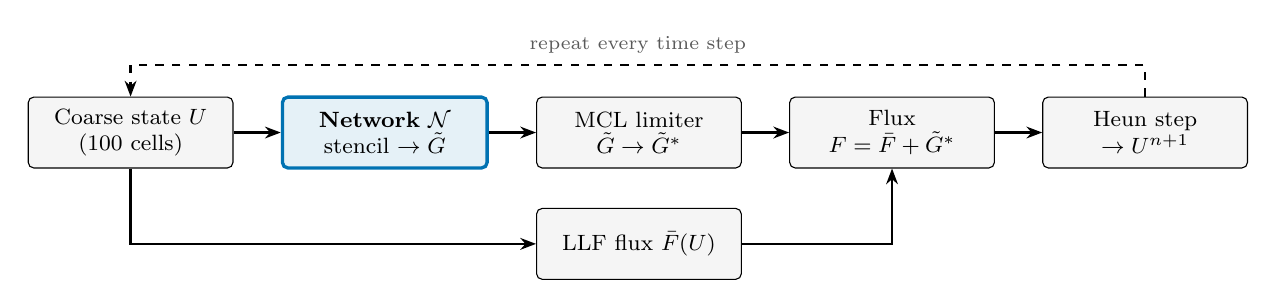
\begin{tikzpicture}[font=\footnotesize,node distance=6mm,
  box/.style={draw,rounded corners=2pt,minimum height=9mm,minimum width=26mm,align=center,fill=gray!8,inner sep=3pt},
  hl/.style={box,fill=oursc!10,draw=oursc,very thick},
  arr/.style={-{Stealth[length=2mm]},thick}]
\node[box](U){Coarse state $U$\\(100 cells)};
\node[hl,right=of U](N){\textbf{Network} $\NN$\\stencil $\to\tilde G$};
\node[box,right=of N](M){MCL limiter\\$\tilde G\to\tilde G^{*}$};
\node[box,right=of M](F){Flux\\$F=\bar F+\tilde G^{*}$};
\node[box,right=of F](H){Heun step\\$\to U^{n+1}$};
\node[box,below=5mm of M](L){LLF flux $\bar F(U)$};
\draw[arr](U)--(N);\draw[arr](N)--(M);\draw[arr](M)--(F);\draw[arr](F)--(H);
\draw[arr](U.south)|-(L.west);\draw[arr](L.east)-|(F.south);
\draw[arr,dashed](H.north)--++(0,4mm)-|(U.north);
\node[font=\scriptsize,gray!70!black,above=4.2mm of $(U.north)!0.5!(H.north)$]{repeat every time step};
\end{tikzpicture}
\caption{One time step of the reduced model. \paper{} and \ours{} share every block; they differ only in the highlighted network.}
\end{figure}

\section{The two architectures}
\begin{figure}[!t]
\centering
\resizebox{\textwidth}{!}{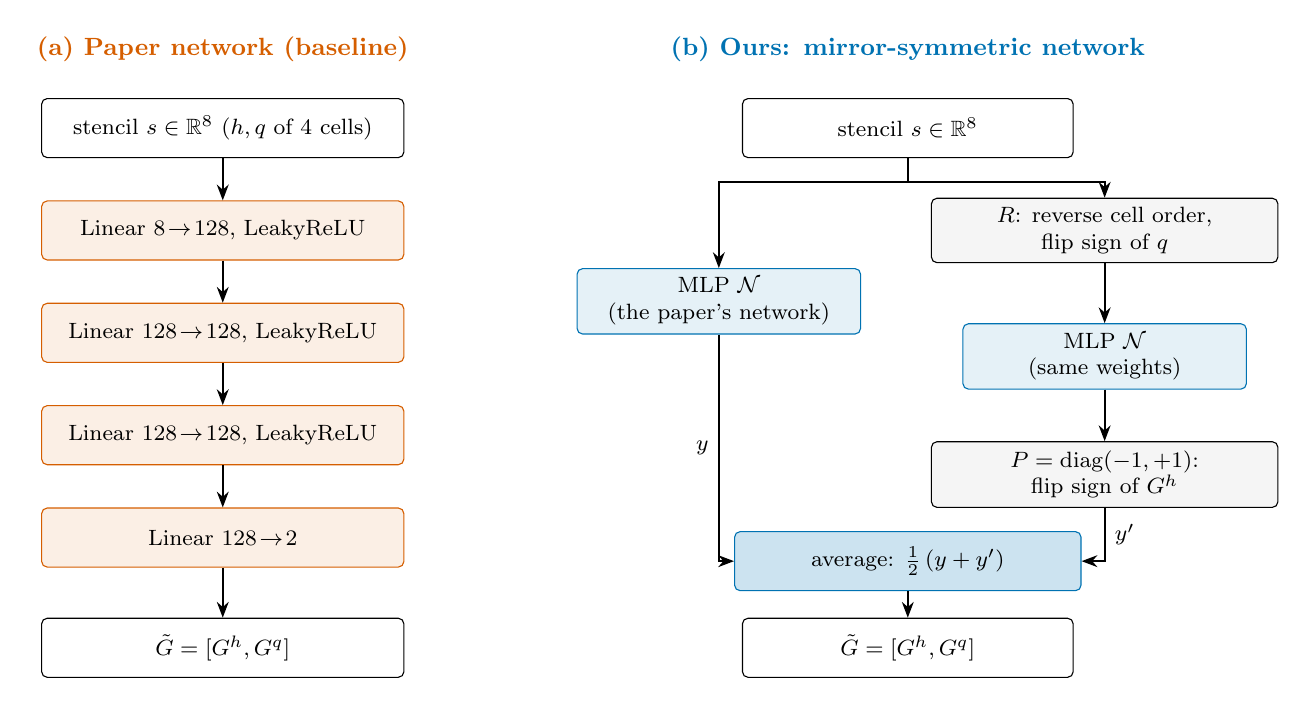
\begin{tikzpicture}[font=\footnotesize,
  lay/.style={draw,rounded corners=2pt,minimum height=7.5mm,align=center,fill=gray!8},
  io/.style={draw,rounded corners=2pt,minimum height=7.5mm,align=center,fill=white},
  arr/.style={-{Stealth[length=2mm]},thick}]
% (a) paper
\node[font=\small\bfseries,text=paperc] at (2.3,1.0){(a) \textbf{Paper} network (baseline)};
\node[io,minimum width=4.6cm](s) at (2.3,0){stencil $s\in\mathbb R^{8}$ ($h,q$ of 4 cells)};
\foreach \i/\t in {1/{Linear $8\!\to\!128$, LeakyReLU},2/{Linear $128\!\to\!128$, LeakyReLU},3/{Linear $128\!\to\!128$, LeakyReLU},4/{Linear $128\!\to\!2$}}
  \node[lay,draw=paperc,fill=paperc!10,minimum width=4.6cm](l\i) at (2.3,{-1.3*\i}){\t};
\node[io,minimum width=4.6cm](g) at (2.3,-6.6){$\tilde G=[G^h,G^q]$};
\draw[arr](s)--(l1);\draw[arr](l1)--(l2);\draw[arr](l2)--(l3);\draw[arr](l3)--(l4);\draw[arr](l4)--(g);
% (b) ours
\node[font=\small\bfseries,text=oursc] at (11.0,1.0){(b) \textbf{Ours}: mirror-symmetric network};
\node[io,minimum width=4.2cm](s2) at (11.0,0){stencil $s\in\mathbb R^{8}$};
\node[lay,draw=oursc,fill=oursc!10,minimum width=3.6cm](nA) at (8.6,-2.2){MLP $\NN$\\(the paper's network)};
\node[lay,minimum width=4.4cm](R) at (13.5,-1.3){$R$: reverse cell order,\\ flip sign of $q$};
\node[lay,draw=oursc,fill=oursc!10,minimum width=3.6cm](nB) at (13.5,-2.9){MLP $\NN$\\(same weights)};
\node[lay,minimum width=4.4cm](P) at (13.5,-4.4){$P=\mathrm{diag}(-1,+1)$:\\ flip sign of $G^h$};
\node[lay,draw=oursc,fill=oursc!20,minimum width=4.4cm](avg) at (11.0,-5.5){average: $\tfrac12\,(y+y')$};
\node[io,minimum width=4.2cm](g2) at (11.0,-6.6){$\tilde G=[G^h,G^q]$};
\draw[arr](s2.south)--++(0,-3mm)-|(nA.north);
\draw[arr](s2.south)--++(0,-3mm)-|(R.north);
\draw[arr](R)--(nB);\draw[arr](nB)--(P);
\draw[arr](nA.south)|-(avg.west)node[pos=.25,left]{$y$};
\draw[arr](P.south)|-(avg.east)node[pos=.25,right]{$y'$};
\draw[arr](avg)--(g2);
\end{tikzpicture}}
\label{fig:arch}
\caption{(a) \paper{}: a plain MLP, 3 hidden layers of 128 neurons. (b) \ours{}: the same MLP, run on the stencil and on its mirror image,
then combined: $\tilde G(s)=\tfrac12\big[\NN(s)+P\,\NN(Rs)\big]$. No extra parameters (the two branches share weights).}
\end{figure}

\textbf{What \ours{} does differently.} If $(h(x),q(x))$ solves the equations then so does its mirror image $(h(-x),-q(-x))$, and the exact subgrid flux transforms
accordingly: $G^h\mapsto -G^h$, $G^q\mapsto G^q$ (we verified this to about $10^{-14}$ on fine-mesh data). The training data only contain flow to the right
($V_0\in[1,2]$), so the \paper{} network has no information about left-moving flow and must extrapolate. The wrapper of Fig.~\ref{fig:arch}(b) enforces the symmetry
\emph{exactly, for any weights}, so what is learned from right-moving flow transfers to left-moving flow. The price is two network evaluations per call.

\begin{table}[!b]
\centering\small
\begin{tabular}{@{}lll@{}}
\toprule & \paper{} (baseline) & \ours{} (extension) \\ \midrule
Inputs / outputs & 8 (4-cell stencil) / 2 ($G^h,G^q$) & same \\
Core network & MLP $3\times128$, LeakyReLU(0.01) & the same MLP \\
Symmetry $x\to-x$ & learned from data only & exact, built in \\
Parameters & 34{,}434 & 34{,}434 (shared) \\
Evaluations per call / cost & 1 / 91\,\textmu s & 2 (batched) / 154\,\textmu s \\
Training samples (train / validation) & 25.6 M / 6.4 M & 12.8 M / 3.2 M \\
Validation loss (standardised units) & $3.96\times10^{-4}$ & $4.37\times10^{-4}$ \\ \bottomrule
\end{tabular}
\caption{Comparison of the two networks. Optimiser, loss, limiter and solver are identical.}
\end{table}

\section{Setup}
\textbf{Training (both).} 200 fine-mesh trajectories of length $T=80$ from random sine initial conditions
($H_0=2$, $V_0\sim U(1,2)$, amplitudes $U(0.2,0.6)$, wavenumbers $1$--$6$), labelled with the exact $G$.
Standardised inputs/outputs, SGD with batch 128 (stage 1: 500 epochs max at lr 0.05; stage 2: 2000 max at lr 0.001), early stopping.
\paper{} used all 32 M samples; \ours{} used every second stored sample (every 20th fine time step, 16 M samples) to stay within the memory of the laptop used.

\textbf{Test cases (20, four categories).}
\emph{Paper cases} (6): Table~1 initial conditions 1--4 of~\cite{timofeyev2025}, a long run to $t{=}400$, and the non-smooth step.
\emph{Outside the training range} (6): depths $H_0=1.25,2.5,3.5$, flows $V_0=4$ and $-1.5$, and a large time step.
\emph{Tough} (5): shallow and near-dry water ($H_0=1.0,0.6$, troughs at $h=0.3$) and two strong dam breaks.
\emph{Method breaks} (3): a medium dam break and very short waves ($k=15,20$, i.e.\ 5--7 coarse cells per wave).

\textbf{Metric.} Relative $\ell^2$ error of $q$ against the 2000-cell reference averaged onto the 100 coarse cells.
Unless stated, the networks run \emph{with} MCL. ``Net alone'' means without the limiter; ``blew up'' means $h<0$.

\section{Results}
\begin{table}[h]
\centering\small\setlength{\tabcolsep}{4pt}
\begin{tabular}{@{}lccccc@{}}
\toprule
Category (cases) & Coarse LLF & \paper{} + MCL & \ours{} + MCL & \ours{} lower in & Net alone blows up \\
 & (no network) & & & (cases) & (\paper{} / \ours{}) \\ \midrule
Paper cases (6) & 2.57\% & \textbf{0.43\%} & 0.58\% & 1 of 6 & 0 / 0 \\
Outside the training range (6) & 5.51\% & 2.45\% & \textbf{1.71\%} & 5 of 6 & 0 / 0 \\
Tough cases (5) & 16.81\% & 8.13\% & \textbf{3.80\%} & 4 of 5 & 5 / 3 \\
Cases where the method breaks (3) & 19.63\% & 13.61\% & \textbf{9.64\%} & 1 of 3 & 0 / 0 \\
\midrule
All cases (20) & 7.78\% & 2.94\% & \textbf{2.41\%} & 11 of 20 & 5 / 3 \\
\bottomrule
\end{tabular}

\caption{Median error of $q$ per category (lower is better; bold = better of the two networks).}
\end{table}

\textbf{Observations.}
\begin{itemize}
\item \textbf{On the paper's cases \paper{} is better} (0.43\% vs 0.58\%; \ours{} wins 1 of 6), consistent with its lower validation loss; both are far better than plain coarse LLF (1.5--7\%).
\item \textbf{Outside the training range \ours{} is better} (1.71\% vs 2.45\%; 5 of 6). The clearest effect is left-moving flow: 4.27\% $\to$ 0.69\%.
\item \textbf{On tough cases \ours{} is better} (3.80\% vs 8.13\%; 4 of 5), e.g.\ the three dam breaks improve by 39--77\%; shallow water $H_0{=}1$ is the exception.
\item \textbf{MCL is essential for both.} The net alone blows up in 5 of 20 cases (\paper{}) and 3 of 20 (\ours{}); with MCL, in none.
\item \textbf{Neither fixes everything.} Dam-break errors remain 3--26\%, and MCL clips real crests of very short waves (error 15\% with MCL vs 2\% without for \paper{}).
\end{itemize}

\begin{figure}[!t]
\centering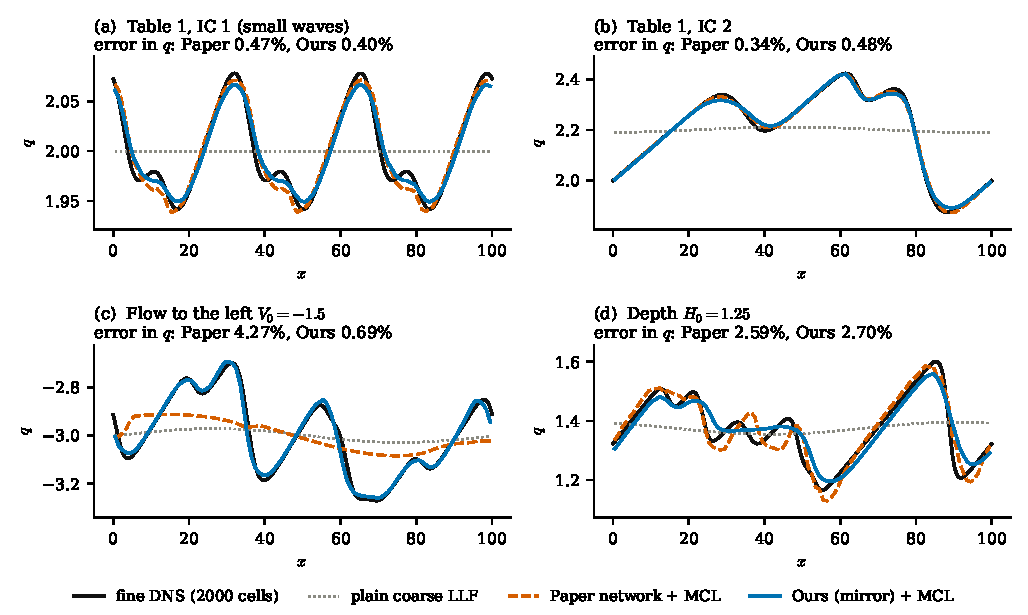
\includegraphics[width=\textwidth]{fig_samples_A.pdf}
\caption{Sample outputs, two cases from each of the first two categories; \textbf{(a,b)} paper cases, \textbf{(c,d)} outside the training range.
Both networks run with MCL. Panel~(b) is a case where \paper{} is better; in (c) the \paper{} network fails on left-moving flow and \ours{} follows the reference; in (d) \paper{} is marginally better.}
\end{figure}

\begin{figure}[!t]
\centering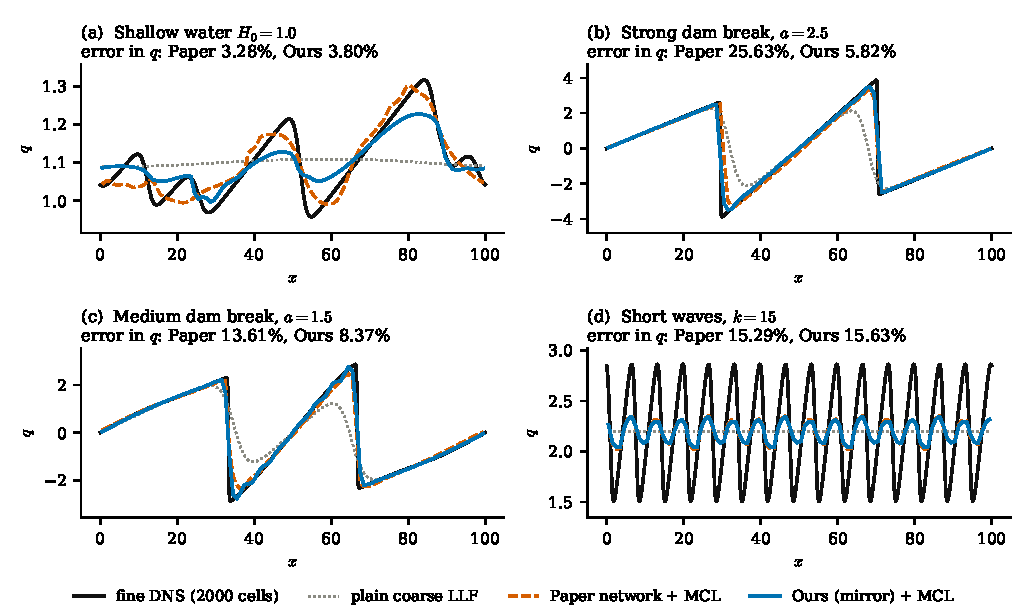
\includegraphics[width=\textwidth]{fig_samples_B.pdf}
\caption{Sample outputs, two cases from each of the last two categories; \textbf{(a,b)} tough cases, \textbf{(c,d)} cases where the method breaks.
Panel~(a) is a case where \paper{} is better; in (b,c) \ours{} resolves the shocks better; in (d) both networks flatten waves resolved by only 7 cells.}
\end{figure}

\section{Limitations and conclusion}
\begin{itemize}
\item \textbf{Unequal training data.} \ours{} saw half the samples; its weaker result on paper cases may partly reflect this. A fair comparison requires retraining it on the full set.
\item \textbf{One trained network each, 20 hand-chosen cases}; no variance over random seeds, so small differences (e.g.\ 0.58\% vs 0.43\%) are not conclusive.
\item \textbf{Speed.} A network call (90--150\,\textmu s in PyTorch) costs more than a full 2000-cell step in NumPy, so the reduced models are faster than the reference only with a larger time step (about 2--5$\times$ at $\Delta T=0.05$).
\item \textbf{Differences from~\cite{timofeyev2025}.} Training uses every 10th fine time step (memory); our Lax--Wendroff baseline (their Fig.~6) is less diffusive than theirs; only the $3\times128$ and $3\times32$ sizes of their size study were trained.
\end{itemize}
\textbf{Conclusion.} The paper's method reproduces as described. Building the exact mirror symmetry into the network is cheap, adds no parameters,
and improves robustness outside the training regime (left-moving flow, deeper or shallower water, dam breaks), at the cost of slightly lower accuracy on the paper's own cases in our (data-limited) experiment.
Code, trained models and an interactive comparison dashboard are in \texttt{work/final\_btp}.

\begin{thebibliography}{9}\small
\bibitem{timofeyev2025} I.~Timofeyev, A.~Schwarzmann, D.~Kuzmin, \emph{Application of machine learning and convex limiting to subgrid flux modeling in the shallow-water equations}, Math.\ Comput.\ Simul.\ \textbf{238} (2025) 163--178.
\end{thebibliography}

\appendix
\section{All 20 test cases}
\begin{table}[H]
\centering\footnotesize
\begin{tabular}{@{}lccccc@{}}
\toprule
Case & Coarse LLF & \paper{} alone & \paper{} + MCL & \ours{} alone & \ours{} + MCL \\ \midrule
\multicolumn{6}{l}{\textit{Paper cases}} \\
Table 1, IC 1 (small waves) & 2.17\% & 0.66\% & 0.47\% & 0.39\% & \textbf{0.40\%} \\
Table 1, IC 2 & 7.00\% & 0.23\% & \textbf{0.34\%} & 0.47\% & 0.48\% \\
Table 1, IC 3 & 1.50\% & 0.42\% & \textbf{0.51\%} & 0.72\% & 0.80\% \\
Table 1, IC 4 & 2.97\% & 0.21\% & \textbf{0.31\%} & 0.38\% & 0.41\% \\
IC 1, long run $t{=}400$ & 1.12\% & 0.66\% & \textbf{0.39\%} & 0.70\% & 0.68\% \\
Step IC, $a{=}0.5$ & 74.10\% & 18.93\% & \textbf{18.53\%} & 21.54\% & 25.15\% \\
\addlinespace
\multicolumn{6}{l}{\textit{Outside the training range}} \\
Depth $H_0{=}2.5$ & 6.19\% & 1.00\% & 1.16\% & 0.79\% & \textbf{1.14\%} \\
Depth $H_0{=}1.25$ & 7.56\% & 4.40\% & \textbf{2.59\%} & 3.13\% & 2.70\% \\
Depth $H_0{=}3.5$ & 7.99\% & 4.69\% & 3.91\% & 3.53\% & \textbf{2.94\%} \\
Fast flow $V_0{=}4$ & 2.59\% & 9.48\% & 1.55\% & 10.64\% & \textbf{1.31\%} \\
Flow to the left $V_0{=}{-}1.5$ & 4.83\% & 3.98\% & 4.27\% & 0.36\% & \textbf{0.69\%} \\
Short waves, $\Delta T{=}0.1$ & 0.68\% & 2.00\% & 2.32\% & 1.23\% & \textbf{2.11\%} \\
\addlinespace
\multicolumn{6}{l}{\textit{Tough cases}} \\
Shallow water $H_0{=}1.0$ & 8.10\% & \textcolor{gray}{\textit{blew up}} & \textbf{3.28\%} & 5.60\% & 3.80\% \\
Very shallow $H_0{=}0.6$ & 16.81\% & \textcolor{gray}{\textit{blew up}} & 9.24\% & \textcolor{gray}{\textit{blew up}} & \textbf{7.12\%} \\
Near-dry troughs, $A_h{=}1.7$ & 9.06\% & \textcolor{gray}{\textit{blew up}} & 1.11\% & \textcolor{gray}{\textit{blew up}} & \textbf{0.89\%} \\
Strong dam break, $a{=}2.5$ & 62.49\% & \textcolor{gray}{\textit{blew up}} & 25.63\% & 12.95\% & \textbf{5.82\%} \\
Dam break into shallow water & 34.57\% & \textcolor{gray}{\textit{blew up}} & 8.13\% & \textcolor{gray}{\textit{blew up}} & \textbf{3.41\%} \\
\addlinespace
\multicolumn{6}{l}{\textit{Cases where the method breaks}} \\
Medium dam break, $a{=}1.5$ & 52.89\% & 22.29\% & 13.61\% & 13.37\% & \textbf{8.37\%} \\
Short waves, $k{=}15$ & 19.63\% & 2.21\% & \textbf{15.29\%} & 4.68\% & 15.63\% \\
Short waves, $k{=}20$ & 11.12\% & 2.79\% & \textbf{9.52\%} & 6.29\% & 9.64\% \\
\bottomrule
\end{tabular}

\caption{Relative $\ell^2$ error of $q$ for every case (bold = better of the two MCL results).}
\end{table}

\end{document}
